%\vspace{-5pt}
\section{Multi-deivce Checkpointing} \label{sec:offline}
%\vspace{-5pt}
%
With the enhanced NVP, REMARK will process the original program with the offline program transformer to pre-set safe checkpoints to collaborate with the new hardware modules to ensure correct online execution.

%\vspace{-5pt}
\subsection{Checkpoint Rules for Multi-device TPC}\label{sec:offlineRules}
\vspace{-5pt}
%
In multi-device systems, we should realize reliable checkpoints considering the processor, the peripherals and the interactions between devices.

As discussed above, a peripheral cannot keep its state when it is interacting with the processor or the environment.
Therefore, \emph{the peripheral checkpoints can only be placed when the peripheral is idle.}
For example, \emph{cp1} and \emph{cp2} in Fig.~\ref{fig:InteractDefine} are two available checkpoints to store the state of the sensor.

In contrast, NVP allows checkpoints at any position in the program and can recover safely.
However, the interaction between processor and peripherals may cause inconsistency.
When power fails during these interactions, the processor may keep its state while the peripheral needs to roll back to a previous position, which leads to inconsistency.
Therefore, \emph{the processor checkpoint should be placed out of the processor-peripheral interaction operations.}

Fig.~\ref{fig:InteractDefine} shows two types of processor-peripheral interactions: I/O operations and interrupts.
First type is I/O operations started by processor to write configurations or commands to peripherals.
Here, if power fails when the processor is configuring or starting the sensor, the processor should rollback to \emph{cp1} or \emph{cp2} to restart the I/O operation.
Second type is the external interrupt activated by peripherals.
Sensor triggers an interrupt when the sensing task is completed, then, the processor read the operation result from the sensor.
If power failure occurs during an interrupt, the processor should not recover the interrupt service routine (ISR).
Instead, it should rollback to \emph{cp3}, the entrance before the interrupt in the main process.
In this way, when the power resumes, ISR is skipped to avoid processing corrupted data in ISR.

Based on these rules, the offline program transformer scans the whole program and inserts safe checkpoints according to the positions of the I/O instructions and the interrupts.

%   
\begin{figure}[t]
    \centering
    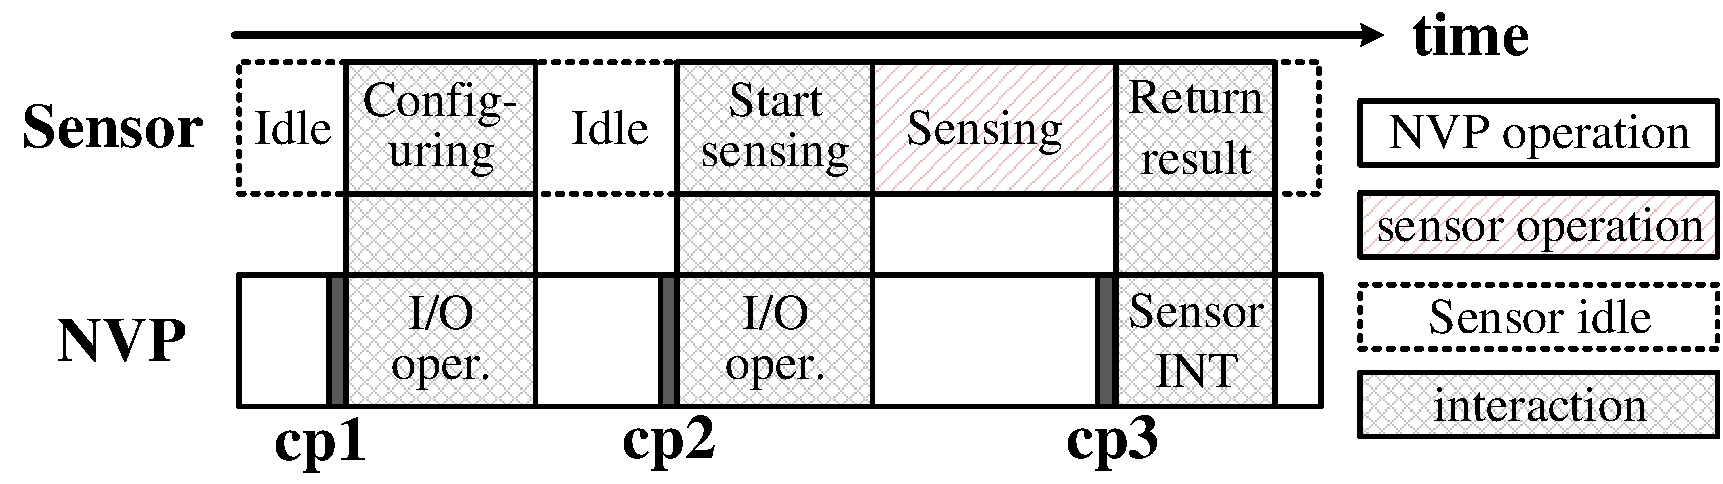
\includegraphics[width=0.48\textwidth]{Fig7_InteractDefine}
    \vspace{-15pt}
    \caption{Interactions between processor and peripheral.}
    \vspace{-5pt}
    \label{fig:InteractDefine}
\end{figure}


\subsection{Offline Program Transformer} \label{sec:offlineTransformer}
\vspace{-5pt}
The offline program transformer contains two steps to handle the I/O instrucitons and the hardware interrupts.

%
\vspace{5pt}
\noindent\textbf{Handle I/O Instructions.} \\
REMARK categorizes I/O instructions into two groups: peripheral configuration instructions and peripheral execution instructions. 
Configuration instructions, including the initialization instructions, are used to configure the internal registers of peripherals.
Execution instructions are used to realize the functionalities of peripherals, such as starting a communication, fetching data from a peripheral buffer, etc. 
Before execution instructions, configuration instructions are required to set the peripherals ready.

%
The pre-processing for I/O instructions involves three steps. 
Fig.~\ref{fig:OfflineStage} shows a data transmission example to illustrate the procedure.
Firstly, REMARK establishes a configuration instruction queue (CFQ) for each peripheral. 
CFQ tracks configuration instructions, including the initialization instructions, of a peripheral, which are used to configure the peripheral in case of power failures.
Every time a new configuration instruction is executed, CFQ will be updated to include the latest configuration modification.

%
To allow REMARK to recognize and pre-process the I/O instructions, the programmers have to implement the peripheral configuration and execution instructions with wrapper functions indicated in the orange parts of Fig.~\ref{fig:OfflineStage}. 
Here, the configuration wrapper function contains the peripheral ID, the target attribute, the configuration value and the pointer of the configuration instruction.
It will execute the configuration instructions and update CFQ with function \emph{\_updateCFQ()}, which will be described in Sec.~\ref{sec:online}.
Execution wrapper function contains the peripheral ID, the peripheral operation ID and the target instruction pointer.
A non-zero peripheral operation ID represents that the instruction starts a peripheral operation.

%
After peripheral related instructions are recognized, two recovering functions are inserted into the program to set checkpoints of processor and peripherals. 
Firstly, a \textbf{checkpoint function} is inserted before each I/O instruction to checkpoint the processor.
With the checkpoint function, the processor rolls back to reconfigure the peripherals to avoid inconsistency.
Second, \textbf{initiator update functions}, \emph{updateInitiator()}, are inserted after the execution instructions of peripheral operations to set peripheral checkpoints.
\emph{updateInitiator(ADD, taskID)} records the start position and the end position of the start program of the peripheral operations, \emph{PT(taskID)}, and adds its peripheral checkpoint into Initiator.
These checkpoints are used to restart the crashed peripheral operations.
Circle 3 and 4 in Fig.~\ref{fig:OfflineStage} (a) illustrates these two functions.
%The details of these two instructions are explained with the recover procedures in Sec.~\ref{sec:online}.

%
\vspace{5pt}
\noindent\textbf{Handle Hardware Interrupts.} \\
Fig.~\ref{fig:OfflineStage} (b) shows the ISR processing procedure with two steps. 
The first step is to set safe checkpoints considering the consistency of processor-peripheral interactions.
Generally, an ISR should not be recovered, if it contains processor-peripheral interactions.
Consider the case that, the embedded volatile memory in a sensor loses all the data after power failure.
If the processor resumes the ISR, it will receive wrong data from the sensor which leads to system errors.
However, ISRs which contain no interactions can be safely recovered after power failure, such as a counter triggered by a timer.
To solve this application specific issue, REMARK provides a control bit, \emph{IR}, to the application developers to indicate whether an ISR can be restored according to application requirements.
Programmers can reset IR, if an ISR is recoverable, or set IR, if it's unrecoverable.
The IR is stored in IRec and the latter can set reliable checkpoints automatically during execution.

The second step is to maintain the peripheral checkpoints.
An interrupt started by a peripheral indicates that the peripheral has completed its task and will enter idle mode.
The system does not need to restart a task if power fails after its completion.
To remove such invalid checkpoint, Initiator update function is inserted at the end of each ISR.
\emph{updateInitiator(REMOVE, taskID)} removes the peripheral checkpoint of \emph{PT(taskID)}.

%
In this way, the program is transformed to be recoverable.
It is now ready to realize recoveries on the proposed hardware. 
Noted that, \emph{programmers can dictate an operation as unrecoverable by not using the wrapper codes according to application-specific reasons, such as data freshness requirements}.

\begin{comment}
\textbf{Optional Recovery Approach}
%
In our design, the integrated master interface of an I/O bus is a non-volatile I/O interface, which utilizes NVFFs to re-initialize and re-configure the I/O bus~\cite{li2016hw}.
No hardware modification is required for the external peripherals. 
The recovery of the operations is optional via software approaches. 
To avoid recovering an operation, the \emph{periTaskID} in the wrapper function as well as the related IR bit is set to zero.

%
The recovery of tasks is application specific and defined by programmers.
However, two kinds of applications are recommended to be recovered to confirm the reliability and achieve higher data acquisition.
First is the applications that rely on hardware interrupts.
Recovering these applications can avoid deadlock caused by un-returned interrupts. 
Second is the normally-off applications requiring frequent 'OFF-ON' switching. 
REMARK realizes fast re-initialization which can improve the data acquisition for long-term periodical data collections.
\end{comment}